\documentclass[a4paper, 11pt]{article}

%author :N. Revéret

%-------------------------------------------------------
% Les packages
%-------------------------------------------------------

\usepackage[T1]{fontenc}
\usepackage[utf8]{inputenc}
\usepackage[french]{babel}
\addto\captionsfrench{\def\tablename{Tableau}}
\addto\captionsfrench{\def\figurename{Figure}}
\usepackage{lmodern}
\usepackage{graphicx} % insertion d'images
\usepackage{tikz} % les graphes
\usetikzlibrary{trees,calc, shapes} % les arbres
\usepackage{lastpage}
\usepackage{caption} % légendes avec deux lignes
\usepackage{booktabs} % Les tableaux

%-------------------------------------------------------
% Dimension de la page
%-------------------------------------------------------
\usepackage[a4paper, total={16cm, 26cm}, includehead, headsep=12pt]{geometry} %taille de la page et marges

%-------------------------------------------------------
% Les entêtes et pied de pages
%-------------------------------------------------------
\usepackage{fancyhdr}
\pagestyle{fancy}
\fancyhf{}
\fancyhead[L]{\scriptsize Spécialité NSI}
\fancyhead[R]{\scriptsize Bac Blanc 2}
\fancyfoot[C]{\scriptsize - $\thepage$ -}
\renewcommand{\headrulewidth}{0.3pt}
\renewcommand{\footrulewidth}{0.3pt}

%-------------------------------------------------------
% La numérotation des questions et des listes
%-------------------------------------------------------
\usepackage[shortlabels]{enumitem}
\setlist[enumerate,1]{parsep= 1em, topsep=0em, partopsep=0em} % les questions sont séparées par une hauteur de ligne
\setlist[enumerate,2]{left=0pt .. \parindent,align=left} % les questions de second niveau débutent sans marge
\setlist[itemize,1]{label=\textbullet} % le label des listes de niveau 1 est un bullet
\setlist[itemize,2]{label=$\circ$} % le label des listes de niveau 2 est un bullet vide
\setlist[itemize,3]{label=$\diamond$} % le label des listes de niveau 3 est un diamant

%-------------------------------------------------------
% Mise en forme du code
%-------------------------------------------------------
\usepackage{listings} 
\usepackage{xcolor}

\definecolor{codegreen}{rgb}{0,0.6,0}
\definecolor{codegray}{rgb}{0.5,0.5,0.5}
\definecolor{codepurple}{rgb}{0.58,0,0.82}
\definecolor{backcolour}{rgb}{0.95,0.95,0.92}

% Le code python
\lstdefinestyle{stylepython}{
	language=Python,
	basicstyle=\ttfamily,
	commentstyle=\color{codegreen},
	keywordstyle=\color{blue},
	stringstyle=\color{olive},
	numberstyle=\tiny,
	frame = single,
	tabsize=2,
	escapeinside = {@}{@},
	breaklines=true,
	breakatwhitespace =true
	}
	
% Le pseudo-code
\lstdefinestyle{stylepseudo}{
	basicstyle=\ttfamily,
	escapeinside = {@}{@},
	frame = single,
	breaklines=true,
	tabsize=2,
	breakatwhitespace =true
	}
	
% Le code bash
\lstdefinestyle{stylebash}{
	basicstyle=\ttfamily,
	escapeinside = {@}{@},
	frame = single,
	breaklines=true,
	tabsize=2,
	breakatwhitespace =true
	}	
			
%-------------------------------------------------------
% Dossier contenant les images
%-------------------------------------------------------
\graphicspath{ {./images/} }


%-------------------------------------------------------
% Distance entre les paragraphes
%-------------------------------------------------------
\setlength{\parskip}{1em}

%-------------------------------------------------------
% Le document
%-------------------------------------------------------
\begin{document}

%-------------------------------------------------------
% La page de titre
%-------------------------------------------------------
\begin{titlepage}
	\newcommand{\HRule}{\rule{\linewidth}{0.5mm}}
	
	\center
	
	\textsc{\large Lycée Saint François-Xavier}\\[0.5cm]
	
	\vfill
	
	\HRule\\[0.5cm]
	
	{\huge\bfseries Spécialité NSI - Bac Blanc 2}
	
	\HRule\\[0.5cm]

	\vfill
	
	\begin{center}
		\fbox{
			\parbox{10cm}{
					\centering Ce sujet comporte {\pageref{LastPage}} pages hormis cette page de titre. \\
					Il faut rendre l'énoncé à l'issue de l'épreuve.
			}
		}
	\end{center}
				
	\vfill

	\makebox[\textwidth]
		{Nom :\enspace\hrulefill}

	\vspace{0.5cm}

	\makebox[\textwidth]
		{Classe:\enspace\hrulefill}
	
	\vfill\vfill
	
	{\large -\,\today\,-}
	
\end{titlepage}

%-------------------------------------------------------
% Exercice 1
%-------------------------------------------------------
{\large{\noindent{\underline{\textbf{Exercice 1:}}}}}

Bertrand est directeur d'une salle de théâtre. Il a reçu l'autorisation d'ouvrir sa salle au public mais en raison 
des contraintes sanitaires il doit s'assurer que deux spectateurs sont toujours séparés par au moins un siège vide.
Cherchant à remplir au maximum chaque rang de fauteuils, Bertrand compte installer les spectateurs une place sur deux.

Amateur de casse-tête, il se pose toutefois une question : dans une rangée de $N$ fauteuils, combien de \textit{dispositions} différentes respectent la condition d'espacement des spectateurs ?

\noindent{\underline{Partie A :} Approche naïve}

Ayant suivi des cours d'informatique, il repense à la représentation binaire des nombres.
Positionner des spectateurs sur un rang de $N$ fauteuils revient à compter combien de nombres de $N$ bits n'ont aucun bits \texttt{1} consécutifs.

Par exemple si $N=3$, les dispositions valides sont représentées par les nombres \texttt{000}, \texttt{001}, \texttt{010}, \texttt{100}, \texttt{101}. Il y en a $5$.

\begin{enumerate}[\underline{\arabic*.}]
	\item Quelles sont les dispositions valides dans le cas où $N=4$ ? Combien y en a-t-il ?
\end{enumerate}

Afin de trouver le nombre de configurations satisfaisantes, Bertrand envisage dans un premier temps de lister tous les nombres de $N$ bits et de ne retenir que ceux satisfaisants la condition.

Afin de vérifier qu'un nombre vérifie bien la condition, il faut s'assurer qu'il ne comporte pas deux bits consécutifs égaux à \texttt{1}.
Après quelques recherches, il établit la règle suivante :
\begin{center}
	\guillemotleft\textit{Dans un nombre entier positif ou  nul} $n$\textit{, le test }\texttt{n \& 2**k == 2**k}\textit{ renvoie }\texttt{True}\\ \textit{si et seulement si le }\texttt{k}\textit{-ième bits de }$n$\textit{ vaut }\texttt{1}\guillemotright
\end{center}

\noindent\textit{\underline{Remarque :}} on numérote les bits de droite à gauche en débutant avec l'indice 0. Ainsi, le bit de rang $1$ de $5$ est \texttt{0} et celui de rang $2$ est \texttt{1} car $5_{10}=101_2$.

Par exemple \texttt{5 \& 2**1 == 2**1} renvoie \texttt{False} alors que \texttt{5 \& 2**2 == 2**2} renvoie \texttt{True}.

\begin{enumerate}[resume*]
	\item \begin{enumerate}[\underline{\alph*.}]
		\item Que renvoie l'appel \texttt{25 \& 2**3 == 2**3} ?
		\item Que renvoie l'appel \texttt{25 \& 2**5 == 2**5} ?
	\end{enumerate}
	\item \'Ecrire en \texttt{python} une fonction \texttt{k\_ieme\_bit} qui prend en argument deux nombres entiers positifs ou nuls \texttt{n} et \texttt{k} et renvoie le \texttt{k}-ième bit de \texttt{n}.
	\item \'Ecrire en \texttt{python} une fonction \texttt{disposition\_valide} qui prend en argument deux nombres entiers positifs ou nuls \texttt{n} et \texttt{maxi} et renvoie \texttt{False} si deux bits consécutifs de \texttt{n} sont égaux à \texttt{1}, \texttt{True} dans le cas contraire. On pourra utiliser la fonction \texttt{k\_ieme\_bit} définie à la question précédente et tester l'égalité des bits de rangs \texttt{0} et \texttt{1}, \texttt{1} et \texttt{2}, $\dots$, \texttt{maxi-1} et \texttt{maxi}.
	\item \begin{enumerate}[\underline{\alph*.}]
			\item Le théâtre de Bertrand propose des rangs de $50$ sièges. Combien de nombres faut-il tester pour répondre au problème ?
			\item Dans l'hypothèse où pour chacun de ces nombres on teste chacun des $50$ bits, combien de tests faut-il effectuer au total sur l'ensemble de tous les nombres ?
		\end{enumerate}
\end{enumerate}

\pagebreak
\noindent{\underline{Partie B :} Programmation dynamique}

Cette approche naïve est donc trop coûteuse. Bertrand décide d'opter pour la \textit{programmation dynamique}.
Son observation initiale est simple : une rangée de $N$ fauteuils n'est rien d'autre qu'une rangée de $N-1$ fauteuils à laquelle on rajoute une place.

Dès lors on peut rencontrer deux cas de figures :
\begin{itemize}
	\item le dernier fauteuil est \textbf{occupé} par un spectateur : dans ce cas l'avant-dernier fauteuil était obligatoirement \textbf{vide}
	\item le dernier fauteuil n'est \textbf{pas occupé} par un spectateur : dans ce cas l'avant-dernier fauteuil était \textbf{vide ou plein}
\end{itemize}

\par Il est dès lors possible de compter le nombre de dispositions satisfaisantes en complétant un tableau comme le tableau \ref{table:dispositions}.

\begin{table}[!ht]
	\begin{center}
		\begin{tabular}{|c|c|c|}
			\toprule
			Fauteuils & Dispositions se terminant & Dispositions se terminant \\
			dans la rangée  & par un siège \textbf{vide} & par un siège \textbf{occupé}\\
			\midrule
			0 & 0 & 0 \\
			1 & 1 & 1 \\
			2 & 2 & 1 \\
			3 & 3 & 2 \\
			\midrule
			4 &   &   \\
			\midrule
			5 &   &   \\
			\bottomrule
		\end{tabular}
		\caption{Nombre de dispositions selon la taille de la rangée}
		\label{table:dispositions}
	\end{center}
\end{table}

\begin{enumerate}[\underline{\arabic*.}]
	\item \begin{enumerate}[\underline{\alph*.}]
			\item Compléter sur cet énoncé les deux dernières lignes du tableau \ref{table:dispositions}.
			\item Combien de dispositions valides existent pour une rangée de $5$ fauteuils ?
	\end{enumerate}
\end{enumerate}

Afin d'écrire un programme permettant de répondre au problème, Bertrand décide de coder le tableau sous forme d'une liste de liste.
Afin de créer un tableau \texttt{T} de \texttt{n+1} lignes et deux colonnes initialement remplies de \texttt{0}, 
il utilise l'instruction \texttt{T = [[0,0] for k in range(n+1)]}.

Dans ce tableau la case de la $n$-ième ligne et de la colonne $0$ (resp. $1$) donne le nombre de dispositions valides se terminant par un siège vide (resp. occupé) pour une rangée de $n$ fauteuils.

Ainsi en reprenant l'exemple du tableau \ref{table:dispositions} on a \texttt{T[3][0] = 3} car il existe $3$ dispositions valides de $3$ sièges se terminant par un siège vide.

De même, puisqu'il existe deux dispositions se terminant par un siège occupé dans une rangée de $3$ fauteuils, on a \texttt{T[3][1] = 2}.

Après avoir initialisé le tableau, Bertrand modifie deux valeurs. En effet il est évident qu'il n'existe qu'une disposition valide se terminant par un fauteuil vide dans une rangée d'un seul fauteuil.
Il en est de même pour la disposition se terminant par un fauteuil occupé. 

\begin{enumerate}[resume*]
	\item Soit $n$ un nombre entier supérieur ou égal à $1$.
	\begin{enumerate}[\underline{\alph*.}]
			\item Justifier que l'on a \texttt{T[n][0] = T[n-1][0] + T[n-1][1]}.
			\item Justifier que l'on a \texttt{T[n][1] = T[n-1][0]}.
	\end{enumerate}
	\item \'Ecrire en \texttt{python} la fonction \texttt{disposition} qui prend en argument le nombre \texttt{n} de fauteuils d'une rangée et qui renvoie le nombre de dispositions valides existant pour cette taille de rangée.
	Cette fonction pourra suivre la démarche suivante :
	\begin{itemize}
		\item Création d'un tableau \texttt{T} de dimensions adaptées initialement rempli de \texttt{0}
		\item Mise à jour des valeurs de \texttt{T} pour la rangée de un fauteuil
		\item Parcours de tous les entiers \texttt{i} entre \texttt{2} et \texttt{n} (inclus) et calcul des valeurs de \texttt{T[i][0]} et \texttt{T[i][1]}
		\item Retour du nombre de dispositions cherché 
	\end{itemize}
\end{enumerate}

\noindent{\underline{Partie C :} Affichage des dispositions valides}

Après avoir réussi à compter les dispositions valides, Bertrand souhaite désormais les afficher.

Pour ce faire il souhaiter écrire en \texttt{python} une fonction \texttt{afficher}. Cette fonction récursive fonctionnera de la manière suivante :
\begin{itemize}
	\item Elle prend en argument un entier \texttt{n} correspondant au nombre de sièges de la rangée et une chaîne de caractères \texttt{dispo} initialement vide
	\item Si la valeur de \texttt{n} est égale à \texttt{0}, elle affiche le contenu de \texttt{dispo}
	\item Sinon, elle teste la valeur de \texttt{dispo} :
		\begin{itemize}
			\item Si cette chaîne est vide ou si son dernier caractère est égal à \texttt{0} elle s'appelle deux fois :
				\begin{itemize}
					\item une première fois avec les arguments \texttt{n-1} et \texttt{dispo+"0"}
					\item une seconde avec les arguments \texttt{n-1} et \texttt{dispo+"1"}
				\end{itemize}
			\item Sinon elle s'appelle avec les arguments \texttt{n-1} et \texttt{dispo+"1"}     
		\end{itemize}
\end{itemize}

\begin{enumerate}[\underline{\arabic*.}]
	\item \'Ecrire le code de la fonction \texttt{afficher}.
\end{enumerate}

%-------------------------------------------------------
% Exercice 2
%-------------------------------------------------------

\vspace{1em}

{\large{\noindent{\underline{\textbf{Exercice 2 :}}}}}

\noindent{\underline{Partie A :} Observation des processus}

Un utilisateur d'un système \textit{linux} utilise la commande \texttt{ps -el}. On rappelle que les options \texttt{-el} indiquent que l'on souhaite lister tous les processus (\texttt{e} pour \textit{every}) et afficher beaucoup d'informations (\texttt{l} pour \textit{long}).

Il obtient le retour ci-dessous :

\begin{figure}[!ht]
	\centering
	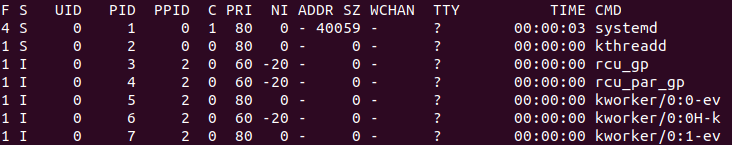
\includegraphics[width=0.9\columnwidth]{ps}
	\centering
	\caption{Sortie de l'appel \texttt{ps -el}}
\end{figure}

\begin{enumerate}[\underline{\arabic*.}]
	\item Que signifie l'acronyme \texttt{PID} ?
	
	\item Que signifie l'acronyme \texttt{PPID} ?
	
	\item Combien de processus sont actuellement en exécution sur cette machine ?
	
\end{enumerate}

\pagebreak
On rappelle les commandes du terminal suivantes :
\begin{itemize}
	\item \texttt{ps -C <commande>} : permet de récupérer le \texttt{PID} du processus associé à la \texttt{<commande>}
	\item \texttt{ps --ppid <PPID>} : permet de lister les processus dont le \texttt{PPID} est égal à \texttt{<PPID>}
\end{itemize}

L'utilisateur effectue donc les commandes suivantes (on fournit aussi les résultats) :

\begin{lstlisting}[style=stylebash]
$ ps -C firefox
2978
$ ps --ppid 2978
PID    TTY    TIME       COMMAND
3379   tty2   00:00:05   Pivileged Cont
3417   tty2   00:00:05   WebExtensions
3455   tty2   00:00:05   Web Content
3501   tty2   00:00:05   Web Content
\end{lstlisting}

\begin{enumerate}[resume*]
	\item Combien de sous-processus ont pour parent le processus associé à \texttt{firefox} ?
\end{enumerate}

La commande \texttt{kill -15 <PID>} permet de terminer un processus désigné par son \texttt{<PID>}.
D'autre part, la documentation de \texttt{firefox} indique que la commande \texttt{Web Content} permet d'ouvrir et de gérer un onglet dans le navigateur.

\begin{enumerate}[resume*]
	\item Quelle commande doit-on saisir dans le terminal afin de fermer le dernier onglet ouvert dans \texttt{firefox} ?
\end{enumerate}

\noindent{\underline{Partie B :} Exécution des processus}

Trois processus $P_1$, $P_2$ et $P_3$ se partagent trois ressources $R_1$, $R_2$ et $R_3$. Dans l'état initial :
\begin{itemize}
	\item[$\bullet$] le processus $P_1$ a obtenu la ressource $R_1$ et demande la ressource $R_2$
	\item[$\bullet$] le processus $P_2$ a obtenu les ressources $R_2$ et $R_3$
	\item[$\bullet$] le processus $P_3$ demande les ressources $R_1$ et $R_3$
\end{itemize}

Cette situation peut être modélisée par le graphe orienté suivant :

\begin{figure}[!ht]
	\centering
	\begin{tikzpicture}[node distance={15mm}, thick]]
		\node[draw, circle, inner sep=0pt, minimum size=8mm] (1) {$R_1$}; 
		\node[draw, rectangle, minimum size=8mm] (2) [right of=1] {$P_1$}; 
		\node[draw, circle, inner sep=0pt, minimum size=8mm] (3) [right of=2] {$R_2$}; 
		\node[draw, rectangle, minimum size=8mm] (4) [below of=1] {$P_3$}; 
		\node[draw, circle, inner sep=0pt, minimum size=8mm] (5) [below of=2] {$R_3$}; 
		\node[draw, rectangle, minimum size=8mm] (6) [below of=3] {$P_2$};
		\draw[->, very thick] (1) -- (2);
		\draw[->, densely dashed] (2) -- (3);
		\draw[->, very thick] (3) -- (6);
		\draw[->, densely dashed] (4) -- (1);
		\draw[->, densely dashed] (4) -- (5);
		\draw[->, very thick] (5) -- (6);
	\end{tikzpicture} 
	\caption{Exemple de relations processus/ressources}
\end{figure}

Dans ce graphe, une arête pointant d'un processus vers une ressource exprime le fait que ce processus demande cette resource.
\textit{A contrario}, une arête pointant d'une ressource vers un processus indique que le processus a obtenu le contrôle de cette ressource pour s'exécuter.

\begin{enumerate}[label=\underline{\arabic*.}]
	\item Proposer, si possible, un ordre d'exécution des processus permettant à la machine de ne pas être bloquée. Justifier.
\end{enumerate}

On considère désormais la situation suivante :
\begin{itemize}
	\item[$\bullet$] Un processus $P_1$ a obtenu la ressource $R_1$ et demande les ressources $R_2$ et $R_3$
	\item[$\bullet$] le processus $P_2$ a obtenu la ressources $R_2$ et demande les ressources $R_3$ et $R_1$
\end{itemize}


\begin{enumerate}[resume*]
	\item \begin{enumerate}[label=\underline{\alph*.}]
			\item Représenter cette situation à l'aide d'un graphe respectant la nomenclature décrite ci-dessus.
			\item Proposer, si possible, un ordre d'exécution des processus permettant à la machine de ne pas être bloquée. Justifier.
			\end{enumerate}
\end{enumerate}

\noindent{\underline{Partie C :} Gestion des priorités}

On s'intéresse à la gestion des priorités des processus.

Une des méthodes possibles est de donner une valeur de \textit{priorité} strictement positive à chaque processus.
Le système d'exploitation exécutera le processus ayant la priorité la plus importante.
On suppose que les processus ont tous des valeurs de priorité différentes les unes des autres.

Il faut donc déterminer facilement quel processus a la priorité la plus grande.
On peut utiliser la structure de \textit{tas-max}.
Cette structure de données est définie ainsi :
\begin{itemize}
	\item un \textit{tas-max} est un arbre binaire
	\item tous les niveaux d'un \textit{tas-max} sont complètement remplis sauf éventuellement le dernier qui est impérativement rempli de gauche à droite
	\item chaque n\oe{}ud a une valeur supérieure à celle de tous ses enfants
\end{itemize}

\begin{figure}[!ht]
	\centering
	\begin{tikzpicture}[level distance=1cm,
		level 1/.style={sibling distance=3cm},
		level 2/.style={sibling distance=1.5cm}]
		\tikzstyle{every node}=[draw,circle, minimum size= 8mm]
		\node {22}
		child {node {20}
		child {node {8}}
		child {node {14}}
		}
		child {node {15}
		child {node {12}}
		child {node [draw=none] {} edge from parent[draw=none]}
		};
	\end{tikzpicture}
	\hspace{1cm}
	\begin{tikzpicture}[level distance=1cm,
		level 1/.style={sibling distance=3cm},
		level 2/.style={sibling distance=1.5cm}]
		\tikzstyle{every node}=[draw,circle, minimum size= 8mm]
		\node {22}
		child {node [fill=lightgray] {23}
		child {node {8}}
			child {node [draw=none] {} edge from parent[draw=none]}
			}
			child {node {15}
		  	child {node {12}}
			  child {node [draw=none] {} edge from parent[draw=none]}
			  };
			\end{tikzpicture}
	\caption{Un \textit{tas-max} à gauche et un contre-exemple à droite}
	\label{fig:tas-max}
\end{figure}

Ainsi dans le contre-exemple de la figure \ref{fig:tas-max}, on observe qu'un des n\oe{}uds ne respecte pas la condition d'ordre et que le dernier rang n'est pas bien construit.

Une telle structure de données peut être implémentée à l'aide d'un tableau dont on numérote les cellules en à partir de l'indice $1$.
Dans ce cadre :
\begin{itemize}
	% Rang de la racine
	\item[$\bullet$] On place la valeur \texttt{0} dans la cellule d'indice $0$. Cette valeur sera ignorée dans les différents traitements
	% Rang de la racine
	\item[$\bullet$] la racine du \textit{tas-max} est dans la cellule d'indice $1$
	\item[$\bullet$] si l'on considère un n\oe{}ud dont la valeur est stockée dans la cellule $n$ :
	\begin{itemize}
			% Rang de la racine
		\item[$-$] la valeur de son fils gauche est stockée dans la cellule $2n$
			% Rang de la racine
			\item[$-$] la valeur de son fils droit est stockée dans la cellule $2n+1$
		\end{itemize}
	\end{itemize}
	
	\newcounter{index}
	\begin{figure}[!ht]
		\centering
		\begin{tikzpicture}
			\setcounter{index}{0}
			\coordinate (s) at (0,0);
		% Rang de la racine
		\foreach \num in {0,22, 20, 15, 8, 14, 12}{
			\node[minimum size=8mm, draw, rectangle] at (s) (\theindex) {\num};
			\node at ($(s)+(0,0.6)$) {\footnotesize \theindex};
			\stepcounter{index}
			\coordinate (s) at ($(s) + (0.8,0)$);
			}
		% Rang de la racine
		\draw [->] (2.south) to [out=-90,in=-90] (4.south);
		% Rang de la racine
		\draw [->] (2.south) to [out=-90,in=-90] (5.south);
	\end{tikzpicture}
	\caption{Représentation du \textit{tas-max} de la figure \ref{fig:tas-max} dans un tableau}
\end{figure}

\begin{enumerate}[label=\underline{\arabic*.}]
	\item \'Ecrire le tableau représentant le \textit{tas-max} de la figure \ref{fig:tas-question}.
\end{enumerate}

\begin{figure}[!ht]
	\centering
	\begin{tikzpicture}[level distance=1cm,
		level 1/.style={sibling distance=3cm},
		level 2/.style={sibling distance=1.5cm}]
		\tikzstyle{every node}=[draw,circle, minimum size=8mm]
		\node {45}
		child {node {40}
		child {node {17} {
			child {node {16}}
			child {node {14}}
			}}
			child {node {28}}
			}
			child {node {30}
			child {node {12}}
			child {node {27}}
			};
		\end{tikzpicture}
		\caption{}
		\label{fig:tas-question}
\end{figure}
	
\begin{enumerate}[resume*]
	\item Dessiner le \textit{tas-max} représenté par le tableau de la figure \ref{fig:tab-question}.
\end{enumerate}
	
\newcounter{indexQuestion}
\begin{figure}[!ht]
	\centering
	\begin{tikzpicture}
		\setcounter{indexQuestion}{0}
		\coordinate (s) at (0,0);
		% Rang de la racine
		\foreach \num in {0,35, 30, 12, 20, 23, 10, 5, 2}{
			\node[minimum size=8mm, draw, rectangle] at (s) (\theindexQuestion) {\num};
			\node at ($(s)+(0,0.6)$) {\footnotesize \theindexQuestion};
			\stepcounter{indexQuestion}
			\coordinate (s) at ($(s) + (0.8,0)$);
			}
		\end{tikzpicture}
		\caption{}
		\label{fig:tab-question}
	\end{figure}
	
	\begin{enumerate}[resume*]
		\item On considère un n\oe{}ud dont la valeur est stockée dans la cellule d'indice $54$ d'un tableau.
		\begin{enumerate}[label=\underline{\alph*.}]
			\item Ce n\oe{}ud est-il le fils gauche ou droit de son père ?
			\item Dans quelle cellule se trouve son père ?
			\item Dans quelle cellule se trouve son grand-père (le père de son père) ?
		\end{enumerate}
	\end{enumerate}
	
Lors de la construction d'un \textit{tas-max}, on commence par ajouter la nouvelle valeur à la fin du tableau.
Cette opération peut rompre la règle d'ordre si cette valeur est supérieure à celle d'au moins un de se ses ascendants.
Il faut dans ce cas \textit{tasser} l'arbre afin de placer la nouvelle valeur à sa place.
Pour ce faire on la fait remonter de proche en proche jusqu'à ce que son parent lui soit supérieur.
	
\begin{figure}[!ht]
	\centering
	\begin{tikzpicture}[level distance=1cm,
		level 1/.style={sibling distance=3cm},
		level 2/.style={sibling distance=1.5cm}]
		\tikzstyle{every node}=[draw,circle, minimum size= 8mm]
		\node {22}
		child {node {20}
		child {node {8}}
		child {node {14}}
		}
		child {node {15}
		child {node {12}}
		child {node [fill=lightgray] {21} edge from parent[draw=none]}
		};
	\end{tikzpicture}
	\hspace{1cm}
	\begin{tikzpicture}[level distance=1cm,
		level 1/.style={sibling distance=3cm},
		level 2/.style={sibling distance=1.5cm}]
		\tikzstyle{every node}=[draw,circle, minimum size= 8mm]
		\node {22}
		child {node {20}
		child {node {8}}
		child {node {14}}
		}
		child {node [fill=lightgray] {21}
		child {node {12}}
		child {node {15}}
		};
	\end{tikzpicture}
	\caption{Insertion de la valeur $21$ dans le \textit{tas-max}}
	\label{fig:insertion}
\end{figure}
		
\begin{enumerate}[resume*]
	\item \'Ecrire le tableau représentant le \textit{tas-max} de la figure \ref{fig:tab-question} après insertion de la valeur 18.
\end{enumerate}

Le pseudo-code de la fonction d'insertion est donné ci-dessous.
Son fonctionnement correspond à celui expliqué plus haut.

% Rang de la racine 
\begin{lstlisting}[style=stylepseudo]
Fonction insertion(tas, valeur) :
	"""
	Ins@è@re la valeur dans le tableau tas repr@é@sentant un tas-max
	Le tableau respecte la condition d'ordre avant l'appel de la fonction
	Renvoie un tableau respectant la condition  l'ordre avec la valeur inser@é@e
	"""
	
	# On ajoute valeur @à@ la fin du tableau
	Ajouter valeur @à@ la fin de tas
	
	# L'indice @é@tudi@é@
	i = longueur(tas) - 1

	Tant que i != 1 et valeur > tas[i//2] : 
		# i//2 est la division enti@è@re
		Echanger les valeurs de tas[i] et tas[i//2]
		i = i // 2
		
	Renvoyer tas
\end{lstlisting}

\begin{enumerate}[resume*]
	\item \'Ecrire le code \texttt{python} de la fonction \texttt{insertion} décrite ci-dessus.
\end{enumerate}

On possède désormais une structure de \textit{tas-max} satisfaisante.
L'élément maximal est donc toujours à l'indice $0$.
Lorsqu'il doit déterminer quel processus exécuter en priorité, le système d'exploitation n'a qu'à piocher ce premier élément.
Plutôt que d'ôter cette valeur du tableau (opération coûteuse car il faudrait "décaler" toutes les autres valeurs d'un cran), on échange cette valeur avec la dernière que l'on supprime.
Cette opération risque toutefois de rompre la structure d'ordre comme indiqué dans la figure \ref{fig:rupture-ordre}.

\newcounter{indexRupture}
\begin{figure}[!ht]
	\centering
	\begin{tikzpicture}
		\setcounter{indexRupture}{0}
		\coordinate (s) at (0,0);
		% Rang de la racine
		\foreach \num in {0, 22, 12, 15, 8, 11, 7}{
			\node[minimum size=8mm, draw, rectangle] at (s) (\theindexRupture) {\num};
			\node at ($(s)+(0,0.6)$) {\footnotesize \theindexRupture};
			\stepcounter{indexRupture}
			\coordinate (s) at ($(s) + (0.8,0)$);
			}
		\end{tikzpicture}
		\hspace{1cm}
		\begin{tikzpicture}[level distance=1cm,
			level 1/.style={sibling distance=3cm},
			level 2/.style={sibling distance=1.5cm}]
			\tikzstyle{every node}=[draw,circle, minimum size= 8mm]
			\node {22}
			child {node {12}
			child {node {8}}
			child {node {11}}
			}
			child {node {15}
			child {node {7}}
			child {node [draw=none] {} edge from parent[draw=none]}
			};
		\end{tikzpicture}
		\par
		\vspace{1em}
		\begin{tikzpicture}
			\setcounter{indexRupture}{0}
			\coordinate (s) at (0.0,0);
		% Rang de la racine
		\foreach \num in {0, 7, 12, 15, 8, 11}{
			\node[minimum size=8mm, draw, rectangle] at (s) (\theindexRupture) {\num};
			\node at ($(s)+(0,0.6)$) {\footnotesize \theindexRupture};
			\stepcounter{indexRupture}
			\coordinate (s) at ($(s) + (0.8,0)$);
			}
			\node[minimum size=8mm, draw, cross out] at (s) (-1) {7};
			% Rang de la racine
			\draw [->] (-1.south) to [out=-130,in=-40] (1.south);
		\end{tikzpicture}
		\hspace{1cm}
		\begin{tikzpicture}[level distance=1cm,
			level 1/.style={sibling distance=3cm},
			level 2/.style={sibling distance=1.5cm}]
			\tikzstyle{every node}=[draw,circle, minimum size= 8mm]
			\node [fill=lightgray] {7}
			child {node {12}
			child {node {8}}
			child {node {11}
			}
			}
			child {node {15}};
		\end{tikzpicture}
		\caption{Un \textit{tas-max} avant et après avoir ôté la valeur maximale}
		\label{fig:rupture-ordre}
	\end{figure}
	
	\begin{enumerate}[resume*]
		\item Compléter sur cet énoncé la fonction \texttt{retablir} ci-dessous écrite en \texttt{python}. 
		Cette fonction prend en argument un tableau codant un \textit{tas-max} dans lequel il est possible que la première valeur rompe l'ordre.
		Il faut alors faire "descendre" cette valeur. La fonction renvoie le tableau \texttt{tas} modifié.
	\end{enumerate}
	
% Rang de la racine
\begin{lstlisting}[style=stylepython, language=Python]
def retablir(tas) :
	# La valeur a descendre
	v = tas[1]
	# l'indice en cours
	i = 1

	# Tant qu'il y a un fils gauche
	while 2*i < ............... :
		# l'indice du fils-gauche 
		i_g =  ...............
		# l'indice du fils-droit
		i_d =  ...............
		# Selection du fils ayant la priorite maximale
		i_max = i_g
		if i_d < len(tas) and tas[i_g] .... tas[i_d] :
			i_max = ...............
		# Si la racine est superieure au fils maximal, on arrete
		if v > tas[i_max] :
			break
		else :
			# on place la valeur d'indice i_max en i
			tas[...............] = tas[...............]
			# On etudie desormais i_max
			i = ...............
	# On place la valeur a descendre en i
	t[i] = v

	# on retourne le tas
	return ...............
\end{lstlisting}

\end{document}